\documentclass[letterpaper, 12pt]{article}
\usepackage{graphicx} % Required for inserting images
\usepackage{textcomp}
\usepackage{fullpage}
\usepackage{amsmath}
\usepackage{xcolor}
\usepackage{float}
\usepackage{geometry}
\usepackage{biblatex}
\geometry{margin=1in}
\usepackage{enumitem}
\usepackage{microtype}
\usepackage{gensymb}
\usepackage{parskip}
\usepackage{tikz}
\usepackage{caption}
\usepackage{cancel}
\usepackage{nicefrac}


\usepackage{hyperref}
\hypersetup{
  colorlinks=true,        % Enable colored links
  linkcolor=teal,         % Set color for internal links
  citecolor=teal,         % Set color for citations
  filecolor=teal,         % Set color for file links
  urlcolor=teal           % Set color for URLs
}

\usepackage[version=4]{mhchem}

\title{Carbohydrates}
\author{BIOS 10016}
\date{24 June 2025}

\begin{document}

\maketitle

\section*{Objectives}

\begin{itemize}
\item Know all definitions presented about Carbohydrates.
\item Classify sugars and describe relationships between sugars based on chemical and structural differences.
\item Use the nomenclature associated with sugar chirality and structure to name sugars in linear and hemiacetal/hemiketal forms.
\item Number the positions in a sugar.
\item Describe the differences between aldoses and ketoses.
\item Describe the properties of the functional groups in sugars, and how it enables them to interact with other molecules, like water.
\item Describe the formation, properties and prevalence of hemiacetal/hemiketal structures of sugars in solution.
\item Interconvert between the Fischer, Projection and Haworth representations.
\item Describe the reactions that sugars undergo:
\begin{itemize}
\item Difference between reducing and non-reducing sugars
\item Isomerization, esterification, and glycoside formation
\item Identify and describe deoxy and amino sugars
\end{itemize}
\item Describe the formation and naming of glycosidic linkages.
\item Identify and name the glycosidic linkages that can exist between sugars.
\item Describe the components, linkages and properties of disaccharides: lactose, maltose, and sucrose.
\item Describe the properties of branched and linear polysaccharides and their
dependence on the types of glycosidic linkages.
\begin{itemize}
\item Differences between starch, amylose, amylopectin and cellulose
\item Difference between amylose and heparin
\end{itemize}
\end{itemize}

\newpage

\section*{Carbohydrates}

\subsection*{Monosaccharides}
\begin{itemize}
\item Monosaccharides are the simplest carbohydrates and are aldehydes or ketones containing two or more hydroxyl groups
\item Aldehyde: aldoses; ketone: ketoses
\item Smallest monosaccharides are composed of 3 carbons
\item End carbon closest to the most oxidized carbon is 1
\item Often represented in \textbf{Fischer} or \textbf{Haworth}
\item Often named relative to glyceraldehyde: D, L (depends on where the hydroxyl group is)
\item D sugars are the most common in nature
\end{itemize}

\subsection*{Chirality}
D and L sugars are defined by the chiral carbon furthest from the most oxidized carbon and where the hydroxyl group is relative to that carbon.

3 carbons - \textbf{triose} \\
4 carbons - \textbf{tetrose} \\
5 carbons - \textbf{pentose} \\
6 carbons - \textbf{hexose}

\subsection*{Different forms of monosaccharides}

\begin{description}
\item [constitutional isomers] same formula, different attachment
\item [stereoisomers] same formula, different 3D orientation
\item [enantiomers] stereoisomers that are nonsuperimposable mirror images of each other (only look at the chiral carbons)
\item [diastereoisomers] stereoisomers that are not mirror images
\item [epimers] diastereoisomers that differ at only one asymmetric carbon atom
\item [anomers] diastereoisomers that differ at a new asymmetric carbon atom formed on ring closure (anomeric carbon (the carbon where the molecule attached differs): $\alpha$ is trans (\ce{CH2OH} and OH on opposite sides), $\beta$ is cis (\ce{CH2OH} and OH on the same side)
\end{description}

\textbf{Hemiacetal} or \textbf{hemiketal} sugars

Aldehyde + alcohol $\to$ hemiacetal \\
Ketone + alcohol $\to$ hemiketal

Happens through \textbf{nucleophilic attack}

$\alpha$ and $\beta$ designations based upon chirality at anomeric carbon

$\alpha$ and $\beta$ conformations are in equilibrium in water. The linear conformation is the least dominant species in solution

\subsection*{Naming of cyclic sugars}
Glucose forms a six-member ring: \textbf{pyranose} since it resembles pyran (most biologically relevant)

Fructose forms a five-member ring: \textbf{furanose} since it resembles furan (most stable)

$\alpha$ and $\beta$ anomers result from carbonyl containing functional groups having two faces.

4 parts to the name:

\begin{enumerate}
\item Anomeric carbon - $\alpha$ or $\beta$?
\item \textcolor{blue}{Chirality - D or L?} (Last carbon pointing up = D, pointing down = L)
\item \textcolor{red}{Sugar name}
\item \textcolor{green}{Number of atoms - furanose or pyranose?}
\end{enumerate}

Example: $\beta$-\textcolor{blue}{D}-\textcolor{red}{Ribo}\textcolor{green}{furanose}

\subsection*{Fischer vs. Haworth Projection}

\begin{itemize}

\item Carbon 1 from the planar structure (carbonyl carbon) becomes anomeric carbon in Haworth projection

\item Last hydroxyl (OH) attacks ketone (C=O) group

\item If O and OH are on same side = cis = $\beta$

\item If O and OH are on opposite sides = trans = $\alpha$

\end{itemize}

\begin{figure}[H]
\centering
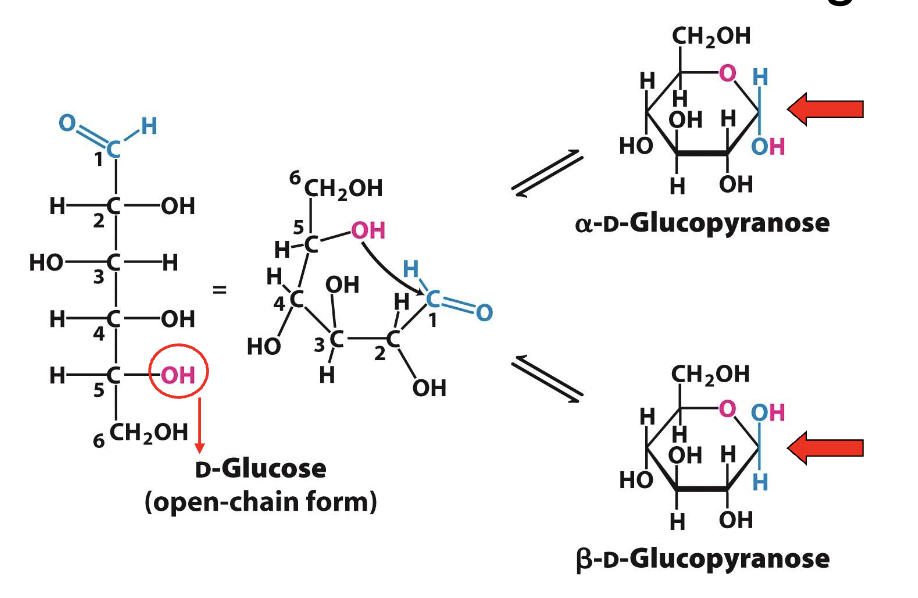
\includegraphics[width=0.8\textwidth]{projections}
\end{figure}

\textbf{To convert from Fischer (open) to Haworth (ring):}

\begin{enumerate}
\item Count the number of carbons - OH attacks C=O (6 membered ring = 5 carbons, 1 oxygen, 5 membered ring = 4 carbons, 1 oxygen)
\item If D, draw the last carbon pointing up; if L, draw the last carbon pointing down
\item Let the Fischer representation fall to the right by 90$\degree$
\item Anything on the original right side should point down
\item Anything on the original left side should point up
\end{enumerate}

\textbf{To convert from Haworth to Fischer:}

\begin{enumerate}
\item Count the number of carbons (even the ones that stick out). Number them. The second carbon is anomeric.
\item Draw out the six-carbon chain.
\item Draw molecules pointing up on the right, and molecules pointing down on the left.
\item Fill in the gaps with hydrogens if the carbon has not fulfilled its octet.
\end{enumerate}

\subsection*{Reducing sugars}
\textbf{Reducing sugars} have an accessible functional group that can be oxidized (the sugar is a reducing agent). Non-reducing sugars cannot be oxidized. Any sugar that can undergo \textbf{ring opening} is a reducing sugar. (hemiacetal, hemiketal, \textbf{free OH group})

Reaction with \textbf{Benedict's solution} or \textbf{Fehling's solution}

\textbf{Benedict's test}: adding 2+ copper ions to a solution containing a reducing sugar will result in a color change from blue to red, indicating the presence of reducing sugars. The sugar will reduce the copper to \ce{Cu2O}.

\subsection*{Reactions}

\subsubsection*{Isomerization reactions}
Fructose can convert to glucose and therefore is a reducing sugar.

Glucose $\rightleftharpoons$ enediol intermediate $\rightleftharpoons$ fructose $\rightleftharpoons$ mannose

\subsubsection*{Esterification reactions}

sugar + fatty acid $\to$ ester \\
sugar + phosphate $\to$ phosphoester \\
glucose-6-phosphate (glycolysis, glycogenesis, and pentose phosphate pathway) \\

Adding phosphate to modify glucose molecules

\subsection*{Sugar derivatives}

\begin{description}
\item [deoxy sugars] monosaccharides with one or more hydroxyl groupsu replaced by hydrogens (constituents of DNA, etc.)
\item [amino sugars] contain an amino group in place of a hydroxyl group, typically at the 2 position
\end{description}

\subsection*{Glycoside formation}
A reaction of the anomeric carbon to form an \textbf{acetal} or \textbf{ketal}

aldehyde + alcohol $\rightleftharpoons$ hemiacetal (OR and OH in the same molecule 2 R groups) $\rightleftharpoons$ acetal (3 R groups and a hydrogen)

ketone + alcohol $\rightleftharpoons$ hemiketal (OR and OH in the same molecule, 3 R groups) $\rightleftharpoons$ ketal (4 R groups)

Under alkaline conditions, reverse reaction does not occur!

If a sugar is a hemiacetal or hemiketal, it is still able to undergo ring opening (a reducing sugar). If a sugar is involved in an acetal or ketal, \textit{it will not be able to undergo ring opening} (not a reducing sugar).

\subsection*{Glycosidic linkages}
Example: $\alpha$-1 reacts with Carbon 6

Named based on the carbons involved ($\alpha$1 $\to$ 6)

Name from the sugar that has the lowest anomeric carbon

\subsection*{Types of sugars}

\subsubsection*{Lactose (milk sugar)}
Combination of \textbf{glucose} and \textbf{galactose} in a glycosidic $\beta$1 $\to$ 4 linkage

Is a reducing sugar

\subsubsection*{Maltose}
An intermediate in starch metabolism

Combination of two glucose molecules in a $\alpha$1 $\to$ 4 glycosidic linkage

\subsubsection*{Amylose}
\textbf{Linear} polymer of glucose molecules, in plants

Has a $\alpha$1 $\to$ 4 glycosidic linkage

Lack of branching enables formation of a helical structure stabilized by H-bonds between hydroxyl groups. Left-handed (\textbf{polysaccharides are usually left-handed})

One of the components of \textbf{starch}

\subsubsection*{Cellulose}
Polymer of \textbf{glucose}, synthesized by plants

Predominantly $\beta$1 $\to$ 4 linkages (not able to be broken down by humans)

Forms sheet-like structures stabilized by H-bonds between hydroxyl groups

\subsubsection*{Amylopectin and glycogen}
Glucose polymer

Predominantly $\alpha$1 $\to$ 4 linkages

Highly branched - $\alpha$1 $\to$ 6 linkages

Technically reducing sugars

Non reducing end is the end of the chain that does not have a free anomeric carbon

Reducing end is the end of the chain that has a free anomeric carbon

\subsection*{Heteroglycans}
Polymers of two or more different monosaccharides

\textbf{Glycosaminoglycans:} polymers of glucosamine or galactosamine derivatives that include a carboxylate or sulfate group

\end{document}